\documentclass[times,t]{beamer}
\usepackage{amssymb}
\usepackage{amsmath}
\usepackage{amsfonts}
\usepackage{lmodern} 
% Calligraphic fonts
\newcommand{\calA}{{\cal A}}
\newcommand{\calB}{{\cal B}}
\newcommand{\calC}{{\cal C}}
\newcommand{\calD}{{\cal D}}
\newcommand{\calE}{{\cal E}}
\newcommand{\calF}{{\cal F}}
\newcommand{\calG}{{\cal G}}
\newcommand{\calH}{{\cal H}}
\newcommand{\calI}{{\cal I}}
\newcommand{\calJ}{{\cal J}}
\newcommand{\calK}{{\cal K}}
\newcommand{\calL}{{\cal L}}
\newcommand{\calM}{{\cal M}}
\newcommand{\calN}{{\cal N}}
\newcommand{\calO}{{\cal O}}
\newcommand{\calP}{{\cal P}}
\newcommand{\calQ}{{\cal Q}}
\newcommand{\calR}{{\cal R}}
\newcommand{\calS}{{\cal S}}
\newcommand{\calT}{{\cal T}}
\newcommand{\calU}{{\cal U}}
\newcommand{\calV}{{\cal V}}
\newcommand{\calW}{{\cal W}}
\newcommand{\calX}{{\cal X}}
\newcommand{\calY}{{\cal Y}}
\newcommand{\calZ}{{\cal Z}}

% Sets:
\newcommand{\setA}{\textsf{A}}
\newcommand{\setB}{\textsf{B}}
\newcommand{\setC}{\textsf{C}}
\newcommand{\setD}{\textsf{D}}
\newcommand{\setE}{\textsf{E}}
\newcommand{\setF}{\textsf{F}}
\newcommand{\setG}{\textsf{G}}
\newcommand{\setH}{\textsf{H}}
\newcommand{\setI}{\textsf{I}}
\newcommand{\setJ}{\textsf{J}}
\newcommand{\setK}{\textsf{K}}
\newcommand{\setL}{\textsf{L}}
\newcommand{\setM}{\textsf{M}}
\newcommand{\setN}{\textsf{N}}
\newcommand{\setO}{\textsf{O}}
\newcommand{\setP}{\textsf{P}}
\newcommand{\setQ}{\textsf{Q}}
\newcommand{\setR}{\textsf{R}}
\newcommand{\setS}{\textsf{S}}
\newcommand{\setT}{\textsf{T}}
\newcommand{\setU}{\textsf{U}}
\newcommand{\setV}{\textsf{V}}
\newcommand{\setW}{\textsf{W}}
\newcommand{\setX}{\textsf{X}}
\newcommand{\setY}{\textsf{Y}}
\newcommand{\setZ}{\textsf{Z}}

% Vectors
\newcommand{\bfa}{\mathbf{a}}
\newcommand{\bfb}{\mathbf{b}}
\newcommand{\bfc}{\mathbf{c}}
\newcommand{\bfd}{\mathbf{d}}
\newcommand{\bfe}{\mathbf{e}}
\newcommand{\bff}{\mathbf{f}}
\newcommand{\bfg}{\mathbf{g}}
\newcommand{\bfh}{\mathbf{h}}
\newcommand{\bfi}{\mathbf{i}}
\newcommand{\bfj}{\mathbf{j}}
\newcommand{\bfk}{\mathbf{k}}
\newcommand{\bfl}{\mathbf{l}}
\newcommand{\bfm}{\mathbf{m}}
\newcommand{\bfn}{\mathbf{n}}
\newcommand{\bfo}{\mathbf{o}}
\newcommand{\bfp}{\mathbf{p}}
\newcommand{\bfq}{\mathbf{q}}
\newcommand{\bfr}{\mathbf{r}}
\newcommand{\bfs}{\mathbf{s}}
\newcommand{\bft}{\mathbf{t}}
\newcommand{\bfu}{\mathbf{u}}
\newcommand{\bfv}{\mathbf{v}}
\newcommand{\bfw}{\mathbf{w}}
\newcommand{\bfx}{\mathbf{x}}
\newcommand{\bfy}{\mathbf{y}}
\newcommand{\bfz}{\mathbf{z}}


\newcommand{\bfalpha}{\boldsymbol{\alpha}}
\newcommand{\bfbeta}{\boldsymbol{\beta}}
\newcommand{\bfgamma}{\boldsymbol{\gamma}}
\newcommand{\bfdelta}{\boldsymbol{\delta}}
\newcommand{\bfepsilon}{\boldsymbol{\epsilon}}
\newcommand{\bfzeta}{\boldsymbol{\zeta}}
\newcommand{\bfeta}{\boldsymbol{\eta}}
\newcommand{\bftheta}{\boldsymbol{\theta}}
\newcommand{\bfiota}{\boldsymbol{\iota}}
\newcommand{\bfkappa}{\boldsymbol{\kappa}}
\newcommand{\bflambda}{\boldsymbol{\lambda}}
\newcommand{\bfmu}{\boldsymbol{\mu}}
\newcommand{\bfnu}{\boldsymbol{\nu}}
\newcommand{\bfomicron}{\boldsymbol{\omicron}}
\newcommand{\bfpi}{\boldsymbol{\pi}}
\newcommand{\bfrho}{\boldsymbol{\rho}}
\newcommand{\bfsigma}{\boldsymbol{\sigma}}
\newcommand{\bftau}{\boldsymbol{\tau}}
\newcommand{\bfupsilon}{\boldsymbol{\upsilon}}
\newcommand{\bfphi}{\boldsymbol{\phi}}
\newcommand{\bfchi}{\boldsymbol{\chi}}
\newcommand{\bfpsi}{\boldsymbol{\psi}}
\newcommand{\bfomega}{\boldsymbol{\omega}}
\newcommand{\bfxi}{\boldsymbol{\xi}}
\newcommand{\bfell}{\boldsymbol{\ell}}

% Matrices
\newcommand{\bfA}{\mathbf{A}}
\newcommand{\bfB}{\mathbf{B}}
\newcommand{\bfC}{\mathbf{C}}
\newcommand{\bfD}{\mathbf{D}}
\newcommand{\bfE}{\mathbf{E}}
\newcommand{\bfF}{\mathbf{F}}
\newcommand{\bfG}{\mathbf{G}}
\newcommand{\bfH}{\mathbf{H}}
\newcommand{\bfI}{\mathbf{I}}
\newcommand{\bfJ}{\mathbf{J}}
\newcommand{\bfK}{\mathbf{K}}
\newcommand{\bfL}{\mathbf{L}}
\newcommand{\bfM}{\mathbf{M}}
\newcommand{\bfN}{\mathbf{N}}
\newcommand{\bfO}{\mathbf{O}}
\newcommand{\bfP}{\mathbf{P}}
\newcommand{\bfQ}{\mathbf{Q}}
\newcommand{\bfR}{\mathbf{R}}
\newcommand{\bfS}{\mathbf{S}}
\newcommand{\bfT}{\mathbf{T}}
\newcommand{\bfU}{\mathbf{U}}
\newcommand{\bfV}{\mathbf{V}}
\newcommand{\bfW}{\mathbf{W}}
\newcommand{\bfX}{\mathbf{X}}
\newcommand{\bfY}{\mathbf{Y}}
\newcommand{\bfZ}{\mathbf{Z}}


\newcommand{\bfGamma}{\boldsymbol{\Gamma}}
\newcommand{\bfDelta}{\boldsymbol{\Delta}}
\newcommand{\bfTheta}{\boldsymbol{\Theta}}
\newcommand{\bfLambda}{\boldsymbol{\Lambda}}
\newcommand{\bfPi}{\boldsymbol{\Pi}}
\newcommand{\bfSigma}{\boldsymbol{\Sigma}}
\newcommand{\bfUpsilon}{\boldsymbol{\Upsilon}}
\newcommand{\bfPhi}{\boldsymbol{\Phi}}
\newcommand{\bfPsi}{\boldsymbol{\Psi}}
\newcommand{\bfOmega}{\boldsymbol{\Omega}}


% Blackboard Bold:
\newcommand{\bbA}{\mathbb{A}}
\newcommand{\bbB}{\mathbb{B}}
\newcommand{\bbC}{\mathbb{C}}
\newcommand{\bbD}{\mathbb{D}}
\newcommand{\bbE}{\mathbb{E}}
\newcommand{\bbF}{\mathbb{F}}
\newcommand{\bbG}{\mathbb{G}}
\newcommand{\bbH}{\mathbb{H}}
\newcommand{\bbI}{\mathbb{I}}
\newcommand{\bbJ}{\mathbb{J}}
\newcommand{\bbK}{\mathbb{K}}
\newcommand{\bbL}{\mathbb{L}}
\newcommand{\bbM}{\mathbb{M}}
\newcommand{\bbN}{\mathbb{N}}
\newcommand{\bbO}{\mathbb{O}}
\newcommand{\bbP}{\mathbb{P}}
\newcommand{\bbQ}{\mathbb{Q}}
\newcommand{\bbR}{\mathbb{R}}
\newcommand{\bbS}{\mathbb{S}}
\newcommand{\bbT}{\mathbb{T}}
\newcommand{\bbU}{\mathbb{U}}
\newcommand{\bbV}{\mathbb{V}}
\newcommand{\bbW}{\mathbb{W}}
\newcommand{\bbX}{\mathbb{X}}
\newcommand{\bbY}{\mathbb{Y}}
\newcommand{\bbZ}{\mathbb{Z}}




\setbeamertemplate{navigation symbols}{}

\title{ECE 417/598: Camera calibration}
\author{Vikas Dhiman.  }
\date{Feb 9, 2022}
\begin{document}
\begin{frame}
  \titlepage
  \footnote{See Hartley  and Zisserman's Multiple   View  Geometry for  details.}
  \end{frame}

  \begin{frame}{Announcements}
    \begin{itemize}
      \item Midterm next Friday.
      \item Will cover everything until today's lecture
      \item I will release Sample exam on Monday
      \item No programming questions. Expect Linear Algebra question though.
        Only the concepts that we have touched in class. 
      \item Grading: compare you answers to the solution.
        \begin{align}
          u \approxeq v (\epsilon) &\equiv | u - v | \le \epsilon \min(|u|, |v|)
          \\
          u \sim v (\epsilon) &\equiv | u - v | \le \epsilon \max(|u|, |v|)
        \end{align}
    \end{itemize}
  \end{frame}
  
  \begin{frame}{Homogeneous representation of lines}
    \[ ax + by + c = 0\]
  \end{frame}

  \begin{frame}{Projective space}
    \[ \bbP^2 = \bbR^3 - \{  (0, 0, 0)^\top \}   \]
    \end{frame}

    \begin{frame}{Homogeneous representation of points}
      \[ ax + by + c = 0\]
    \end{frame}

\begin{frame}{Eq of line in Projective space}
      The point $\bfx \in \bbP^2$ lies on a line $\bfl$ if and only if
      $\bfx^\top \bfl = 0$.
\end{frame}


\begin{frame}{Points are rays and  lines are  planes}
  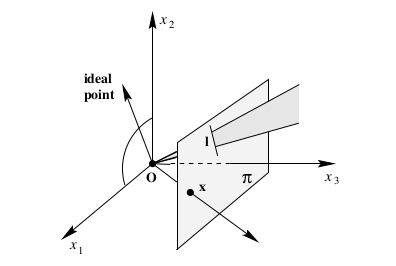
\includegraphics[width=\linewidth]{media/projective-plane-points-are-rays-and-lines-are-planes.png}
\end{frame}

\begin{frame}{Intersection of lines}
\end{frame}


\begin{frame}{Intersection  of  parallel  lines}
  Find   the  intersection  of  parallel lines  $ax+by+c =  0$  and  $ax+by+c'=0$.
\end{frame}

\begin{frame}{Numerical example}
  Find   the  intersection  of  $x =  1$  and  $y=1$ using  perspective  geometry.
\end{frame}

\begin{frame}{Line joining  points}
\end{frame}

\begin{frame}{Homography}
  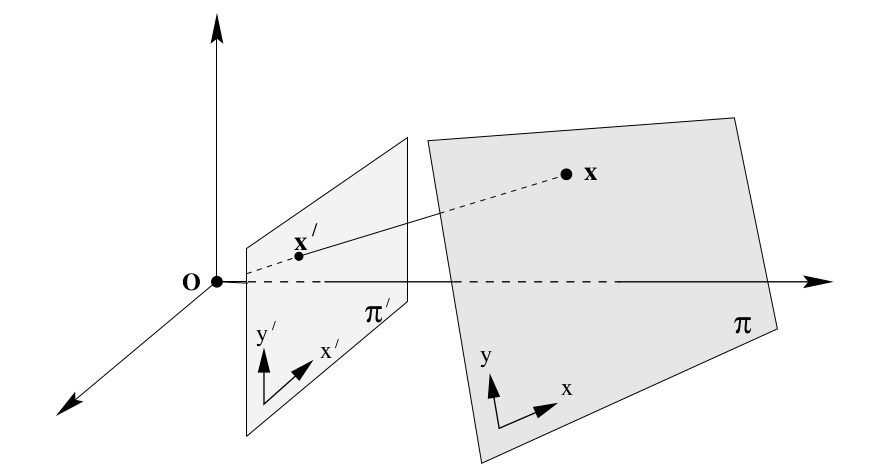
\includegraphics[width=\linewidth]{media/homography-maps-a-line-to-a-line.png}
\end{frame}

\begin{frame}{Examples  of  Homography}
  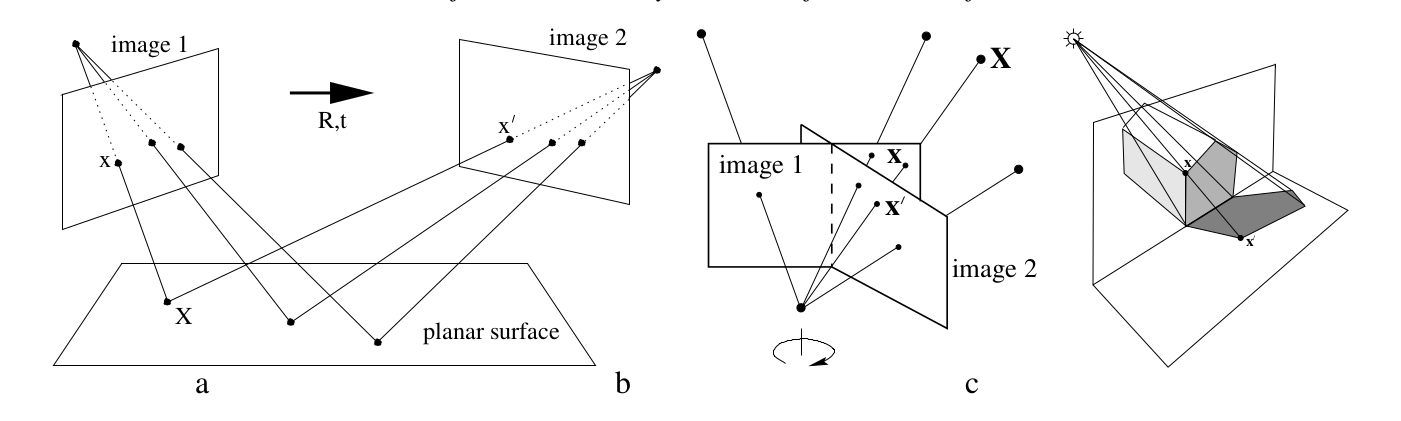
\includegraphics[width=\linewidth]{media/examples-of-homography.png}
\end{frame}

\begin{frame}{Computing Homography}
  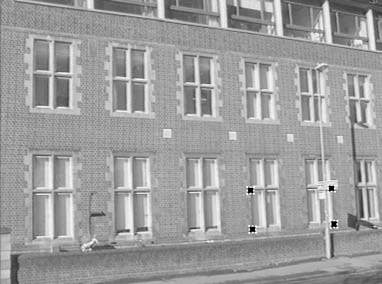
\includegraphics[width=0.45\linewidth]{media/removing-perspective-distortion.png}
  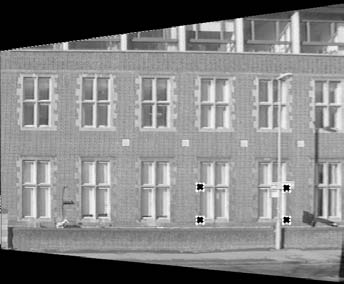
\includegraphics[width=0.45\linewidth]{media/removing-perspective-distortion-b.png}
\end{frame}
\begin{frame}
  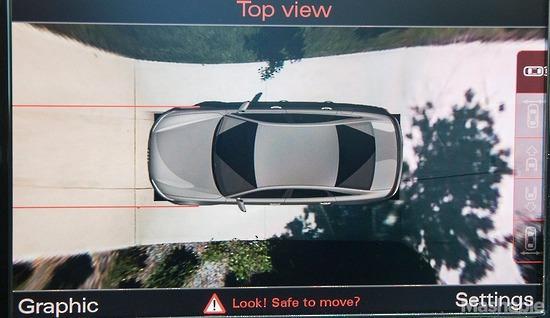
\includegraphics[width=0.60\linewidth]{media/audi top view camera.jpg}
\end{frame}

\begin{frame}{2D homography}
Given a set of points $\bfx_i \in \bbP^2$ and a corresponding set of
points $\bfx'_i \in \bbP^2$, compute the projective transformation that takes each
$\bfx_i$ to $\bfx'_i$ . In a practical situation, the points $\bfx_i$ and   $\bfx'_i$  are points in two images
(or the same image), each image being considered as a projective plane  $\bbP^2$.
\end{frame}

\begin{frame}{Direct Linear Transformation   (DLT) algorithm}
  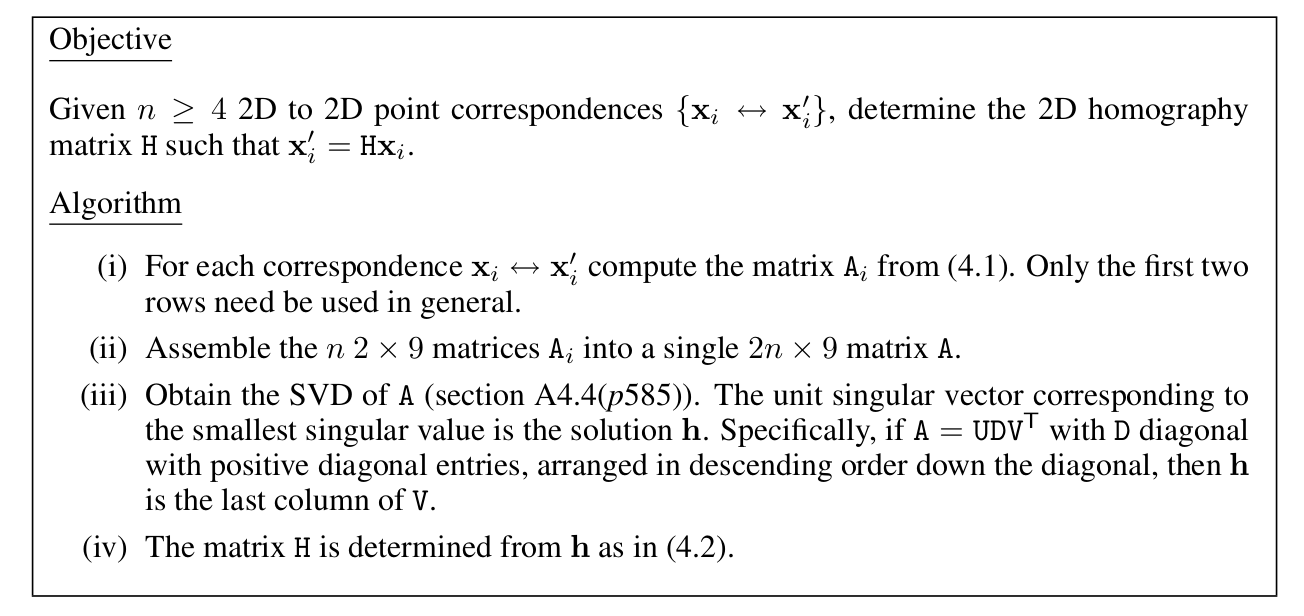
\includegraphics[width=\linewidth]{media/DLT-algorithm.png}
\end{frame}

\begin{frame}{3D  to  2D camera projection matrix estimation}
  Given a set of points $\bfX_i$ in 3D space, and a set
  of corresponding points $\bfx_i$ in an image, find the 3D to 2D projective
  $\bfP$ mapping
  that maps $\bfX_i$ to $\bfx_i  =  \bfP\bfX_i$.
  \end{frame}

\begin{frame}{Eigenvalues  and Eigenvectors}

For a  square  matrix $A$, the $\lambda_i$ and  $\bfx_i$ that satisfy  the
following equation are called eigenvalues and  eigenvectors  respectively.
\begin{align}
  A  \bfx &= \lambda \bfx \text{ or } (A  - \lambda I)\bfx  = 0
\end{align}

$\lambda$ is   chosen to ensure  that   $A  -  \lambda I$  has null space,
hence, characteristic   equation
\begin{align}
  \det(A  - \lambda I) = 0 
 \end{align}

 For  symmetrix matrix $A =  A^\top$, eigenvalues  are  real, and eigenvectors
 are orthonormal,
 \begin{align}
   &A[\bfx_1, \dots,   \bfx_n]  = [\bfx_1, \dots,   \bfx_n]\begin{bmatrix}\lambda_1 &   \dots   &  0 \\
     \vdots   &   \ddots &  \vdots \\
   0 &   \dots  &  \lambda_n \end{bmatrix}
                  \\
   &A  S = S  \Lambda
   \\
   &\text{  if   }  A =  A^\top \text{ then   }  A   = S \Lambda S^\top
   \end{align}


\end{frame}

\begin{frame}{Singular Value  Decomposition (SVD)}
  \begin{align}
    A  &=   U  \begin{bmatrix}\Sigma   &  0  \\   0  &  0 \end{bmatrix} V^\top \\
    A^\top A &= V \Sigma^2  V^{-1} \\
    A^\top A \bfv_i  &= \lambda_i \bfv_i & \lambda_i = \sigma_i^2\\
    A V   &= U \begin{bmatrix}\Sigma   &  0  \\   0  &  0 \end{bmatrix}\\
    U^+   &=  \Sigma^{-1}AV^+
    \end{align}
\end{frame}

\end{document}